\documentclass[11pt]{article}
\usepackage[margin=0.8in]{geometry}
\usepackage{amsmath, amssymb}
\usepackage{booktabs}
\usepackage{array}
\usepackage{enumitem}
\usepackage{fancyhdr}
\usepackage{parskip}
\usepackage{bm}
\usepackage{tikz}
\usetikzlibrary{shapes,arrows,positioning,calc}

% Header and Footer
\pagestyle{fancy}
\fancyhf{}
\setlength{\headheight}{13.6pt}
\fancyhead[C]{\textbf{Chapter 1: Sampling and Descriptive Statistics Summary Notes}}
\fancyfoot[C]{CEE 305 - Spring 2026}
\renewcommand{\headrulewidth}{1pt}
\renewcommand{\footrulewidth}{0.5pt}

\begin{document}

% ==========================================
\section*{Why Statistics?}
% ==========================================
Statistics helps us:
\begin{itemize}[nosep]
    \item Deal with uncertainty in repeated scientific measurements
    \item Draw conclusions from data
    \item Design valid experiments and draw reliable conclusions
    \item Become well-informed members of society
\end{itemize}

\section*{The Core Problem: Samples vs. Populations}
\begin{quote}
\textbf{Key Insight:} We often cannot measure an entire population, so we take a sample and use it to make inferences about the population. The sample rarely perfectly represents the population—this is where statistics helps us quantify the uncertainty.
\end{quote}

\textbf{Example:} A quality engineer wants to know how many of 1000 steel rods meet specifications. Measuring all 1000 is impractical, so he samples 50 rods and finds 46 (92\%) meet specs. Questions that arise:
\begin{enumerate}[nosep]
    \item How large is a typical sampling difference?
    \item What interval gives a good estimate of the population percentage?
    \item How certain can we be that at least 90\% of all rods are good?
\end{enumerate}

% ==========================================
\section*{Section 1.1: Sampling}
% ==========================================
\subsection*{Fundamental Definitions}
\begin{itemize}[nosep]
    \item \textbf{Population:} The entire collection of objects or outcomes about which information is sought.
    \item \textbf{Sample:} A subset of a population, containing the objects or outcomes that are actually observed.
    \item \textbf{Simple Random Sample (SRS):} A sample of size \(n\) chosen by a method in which each collection of \(n\) population items is equally likely to comprise the sample.
\end{itemize}

\textbf{How to obtain an SRS:}
\begin{enumerate}[nosep]
    \item Assign a number to each member of the population
    \item Use a random number generator to select \(n\) numbers
    \item The corresponding items form the sample
\end{enumerate}

\subsection*{Sample of Convenience}
\begin{quote}
\textbf{Definition:} A sample of convenience is a sample that is \textbf{not} drawn by a well-defined random method.
\end{quote}
\textbf{Warning:} Convenience samples may differ systematically from the population. Use them only when random sampling is infeasible, and always think carefully about potential biases.

\subsection*{Sampling Variation}
\begin{quote}
\textbf{Definition:} Sampling variation is the phenomenon where different samples from the same population differ from each other and from the population.
\end{quote}

\subsection*{Types of Populations}
\begin{itemize}[nosep]
    \item \textbf{Tangible Populations:} Consist of physical objects (students, bolts, etc.); always finite.
    \item \textbf{Conceptual Populations:} Consist of all values that might possibly have been observed (e.g., all possible scale readings); often infinite.
\end{itemize}

\subsection*{Independence}
Items in a sample are independent if knowing the values of some items does not help predict the values of others. Items in an SRS may be treated as independent unless the sample comprises more than about 5\% of a finite population.

\subsection*{Other Sampling Methods}
Weighted sampling, stratified random sampling, cluster sampling.

\subsection*{Experiments vs. Observational Studies}
\begin{itemize}[nosep]
    \item \textbf{Controlled experiment:} Experimenter controls factors; can establish cause-and-effect.
    \item \textbf{Observational study:} Experimenter merely observes; cannot reliably establish causation.
\end{itemize}

% ==========================================
\section*{Variables and Data}
% ==========================================
\begin{itemize}[nosep]
    \item \textbf{Variable:} A characteristic that changes over time or among individuals.
    \item \textbf{Experimental unit:} The object on which a variable is measured.
    \item \textbf{Measurement:} The result when a variable is measured on a unit.
    \item \textbf{Data:} A set of measurements.
\end{itemize}

\subsection*{Data Classification by Number of Variables}
Univariate (one variable), bivariate (two variables), multivariate (more than two).

\subsection*{Types of Data}
\begin{itemize}[nosep]
    \item \textbf{Quantitative (numerical):} Height, weight, age.
    \item \textbf{Categorical (qualitative):} Hair color, zip code, mix type.
\end{itemize}

\subsection*{Types of Quantitative Variables}
\begin{itemize}[nosep]
    \item \textbf{Discrete:} Finite or countable values (e.g., number of defects).
    \item \textbf{Continuous:} Any value in an interval (e.g., height, time).
\end{itemize}

% ==========================================
\section*{Section 1.2: Summary Statistics}
% ==========================================
\subsection*{Sample Mean}
\[
\overline{X} = \frac{1}{n}\sum_{i=1}^{n} X_i
\]

\subsection*{Sample Variance}
\[
s^2 = \frac{1}{n-1}\sum_{i=1}^{n}(X_i-\overline{X})^2 = \frac{1}{n-1}\left(\sum X_i^2 - n\overline{X}^2\right)
\]

\subsection*{Sample Standard Deviation}
\[
s = \sqrt{s^2}
\]

\subsection*{Linear Transformations}
If \(Y_i = a + bX_i\) then \(\overline{Y}=a+b\overline{X}\), \(s_Y^2=b^2 s_X^2\), \(s_Y=|b|s_X\).

\subsection*{Outliers}
Points much larger or smaller than the rest. Do not delete without careful thought.

\subsection*{Median}
Order data; if \(n\) odd, median is middle value; if \(n\) even, average of two middle values. Resistant to outliers.

\subsection*{Quartiles and IQR}
\begin{itemize}[nosep]
    \item \(Q_1\) = 25th percentile, \(Q_3\) = 75th percentile.
    \item \(IQR = Q_3 - Q_1\) (spread of middle 50\%).
\end{itemize}

\subsection*{Percentiles}
The \(p\)th percentile splits data so that \(p\%\) are less and \((100-p)\%\) are greater.

\subsection*{Mode}
The most frequent value.

\subsection*{Sample Statistics vs. Population Parameters}
\begin{itemize}[nosep]
    \item \textbf{Statistic:} Numerical summary of a sample (\(\overline{X}, s\)).
    \item \textbf{Parameter:} Numerical summary of a population (\(\mu, \sigma\)).
\end{itemize}

Population mean: \(\mu = \frac{1}{N}\sum_{i=1}^{N} X_i\) (or \(E[X]\)).\\
Population variance: \(\sigma^2 = \frac{1}{N}\sum (X_i-\mu)^2 = E[(X-\mu)^2]\).\\
Population standard deviation: \(\sigma = \sqrt{\sigma^2}\).

\subsection*{Summary Statistics for Categorical Data}
Frequency, relative frequency (\(=\text{frequency}/n\)), percent (\(=100\times\text{relative frequency}\)).

% ==========================================
\section*{Section 1.3: Graphical Summaries}
% ==========================================
\subsection*{Stem-and-Leaf Plot}
Splits each value into a stem (left digits) and leaf (next digit). Displays all data and shape.

\subsection*{Dotplot}
Each data point represented by a dot above a number line. Good for small samples.

\subsection*{Histogram}
Bars that touch; height = frequency or relative frequency. Use 5–12 intervals of equal width.

\subsection*{Describing Distribution Shape}
\begin{itemize}[nosep]
    \item \textbf{Symmetric:} Mirror image about center.
    \item \textbf{Right-skewed:} Long right tail, mean > median.
    \item \textbf{Left-skewed:} Long left tail, mean < median.
    \item \textbf{Unimodal/Bimodal/Multimodal:} Number of peaks.
\end{itemize}

\subsection*{Boxplot}
Box from \(Q_1\) to \(Q_3\) with line at median; whiskers to largest/smallest non-outlier; outliers plotted individually. Fences: \(Q_1-1.5\times IQR\) and \(Q_3+1.5\times IQR\).

\begin{center}
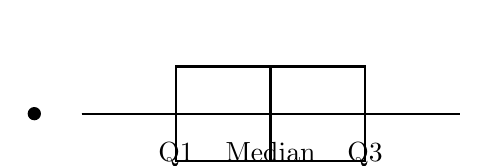
\begin{tikzpicture}[scale=1.2]
\draw[thick] (1,0) -- (5,0);
\draw[thick] (2,-0.5) rectangle (4,0.5);
\draw[thick] (3,-0.5) -- (3,0.5);
\draw[thick] (1,0) -- (2,0);
\draw[thick] (4,0) -- (5,0);
\fill (0.5,0) circle (2pt);
\node at (2,-0.2) [below] {Q1};
\node at (3,-0.2) [below] {Median};
\node at (4,-0.2) [below] {Q3};
\end{tikzpicture}
\end{center}

\subsection*{Scatterplot (for Bivariate Data)}
Each point \((x,y)\) represents a pair. Patterns: positive/negative/no relationship, linear/nonlinear.

\begin{center}
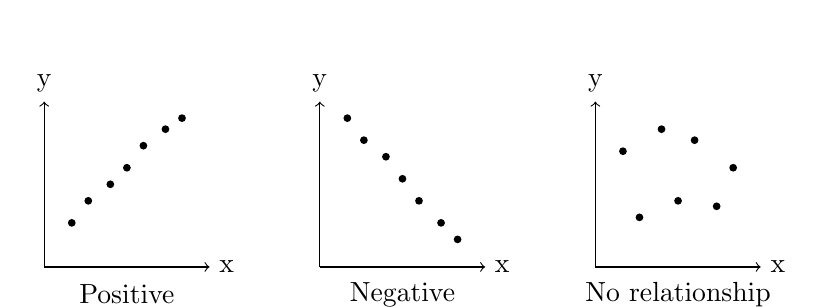
\begin{tikzpicture}[scale=0.7]
\begin{scope}[xshift=0cm]
\draw[->] (0,0) -- (3,0) node[right] {x};
\draw[->] (0,0) -- (0,3) node[above] {y};
\foreach \x/\y in {0.5/0.8,0.8/1.2,1.2/1.5,1.5/1.8,1.8/2.2,2.2/2.5,2.5/2.7} \fill (\x,\y) circle (2pt);
\node at (1.5,-0.5) {Positive};
\end{scope}
\begin{scope}[xshift=5cm]
\draw[->] (0,0) -- (3,0) node[right] {x};
\draw[->] (0,0) -- (0,3) node[above] {y};
\foreach \x/\y in {0.5/2.7,0.8/2.3,1.2/2.0,1.5/1.6,1.8/1.2,2.2/0.8,2.5/0.5} \fill (\x,\y) circle (2pt);
\node at (1.5,-0.5) {Negative};
\end{scope}
\begin{scope}[xshift=10cm]
\draw[->] (0,0) -- (3,0) node[right] {x};
\draw[->] (0,0) -- (0,3) node[above] {y};
\foreach \x/\y in {0.5/2.1,0.8/0.9,1.2/2.5,1.5/1.2,1.8/2.3,2.2/1.1,2.5/1.8} \fill (\x,\y) circle (2pt);
\node at (1.5,-0.5) {No relationship};
\end{scope}
\end{tikzpicture}
\end{center}

% ==========================================
\section*{Summary Table of Key Concepts}
% ==========================================
{\small
\begin{center}
\begin{tabular}{l l}
\toprule
\textbf{Concept} & \textbf{Key Idea} \\
\midrule
Population & Entire collection of interest \\
Sample & Subset actually observed \\
SRS & Every subset equally likely \\
Sampling variation & Samples differ from each other \\
Mean (\(\overline{X}\)) & Arithmetic average \\
Median & Middle value (resistant to outliers) \\
Variance (\(s^2\)) & Average squared deviation from mean \\
Standard deviation (\(s\)) & Typical distance from mean \\
Quartiles & Divide data into quarters \\
IQR & \(Q_3 - Q_1\) (middle 50\% spread) \\
Outlier & Value far from rest of data \\
Parameter & Population summary (\(\mu, \sigma\)) \\
Statistic & Sample summary (\(\overline{X}, s\)) \\
\bottomrule
\end{tabular}
\end{center}
}

% ==========================================
\section*{Definition of Symbols}
% ==========================================
{\small
\begin{center}
\begin{tabular}{l l}
\toprule
\textbf{Symbol} & \textbf{Definition} \\
\midrule
\(n\) & Sample size \\
\(X_i\) & \(i\)th measurement in a sample \\
\(\overline{X}\) & Sample mean \\
\(s^2\) & Sample variance \\
\(s\) & Sample standard deviation \\
\(\mu\) & Population mean \\
\(\sigma^2\) & Population variance \\
\(\sigma\) & Population standard deviation \\
\(Q_1\) & First quartile (25th percentile) \\
\(Q_3\) & Third quartile (75th percentile) \\
\(IQR\) & Interquartile range (\(Q_3-Q_1\)) \\
\(p\)th percentile & Value below which \(p\%\) of data fall \\
\(a, b\) & Constants (linear transformation) \\
\(N\) & Population size (tangible population) \\
\bottomrule
\end{tabular}
\end{center}
}

% ==========================================
\section*{Key Terminology}
% ==========================================
\begin{itemize}[nosep]
    \item \textbf{Population:} Entire set of interest.
    \item \textbf{Sample:} Subset actually observed.
    \item \textbf{Simple Random Sample (SRS):} Each subset of size \(n\) equally likely.
    \item \textbf{Sampling variation:} Natural differences among samples.
    \item \textbf{Statistic:} Numerical summary of a sample.
    \item \textbf{Parameter:} Numerical summary of a population.
    \item \textbf{Outlier:} Unusually large or small observation.
    \item \textbf{Skewness:} Asymmetry in the distribution tail.
    \item \textbf{Boxplot:} Graphical summary showing median, quartiles, and outliers.
    \item \textbf{Histogram:} Bar chart of frequencies for grouped data.
\end{itemize}

% ==========================================
\section*{Important Notes}
% ==========================================
\begin{itemize}[nosep]
    \item Always examine data graphically before calculating numerical summaries.
    \item The median is preferred over the mean for skewed distributions or when outliers are present.
    \item The standard deviation \(s\) is always non‑negative; \(s=0\) only when all data are identical.
    \item When the sample size is more than 5\% of a finite population, the independence assumption may be violated.
    \item Outliers should never be deleted automatically; investigate their source.
    \item For categorical data, only frequency tables and bar charts (or pie charts) are appropriate—not means or standard deviations.
    \item The IQR is a robust measure of spread, unaffected by outliers.
\end{itemize}

\end{document}